
\documentclass[letterpaper,times,numbered,print,custommargin]{Classes/PhDThesisPSnPDF}
% ******************************************************************************
% ******************************* Class Options ********************************
% *********************** See README for more details **************************
% ***   https://github.com/kks32/phd-thesis-template/blob/master/README.md   ***
% ******************************************************************************


% ********************************** Preamble **********************************
% Preamble: Contains packages and user-defined commands and settings
% ******************************************************************************
% ****************************** Custom Margin *********************************

% Add `custommargin' in the document class options to use this section
% Set {innerside margin / outerside margin / topmargin / bottom margin}  and
% other page dimensions
\ifsetMargin
\else
% \RequirePackage[left=37mm,right=30mm,top=35mm,bottom=30mm]{geometry}
    \RequirePackage[left=30mm,right=20mm,top=30mm,bottom=20mm]{geometry}
    \setFancyHdr % To apply fancy header after geometry package is loaded
\fi

% % *****************************************************************************
% % ******************* Fonts (like different typewriter fonts etc.)*************
% 
% % Add `customfont' in the document class option to use this section
% \ifsetFont
% \else
%     % Set your custom font here and use `customfont' in options. Leave empty to
%     % load computer modern font (default LaTeX font).  
%     \RequirePackage{libertine} 
% \fi

% *****************************************************************************
% *************************** Bibliography  and References ********************

%\usepackage{cleveref} %Referencing without need to explicitly state fig /table

% Add `custombib' in the document class option to use this section
\ifsetBib % True, Bibliography option is chosen in class options
\else % If custom bibliography style chosen then load bibstyle here
    \RequirePackage[square, sort, numbers, authoryear]{natbib} % CustomBib
\fi

% changes the default name `Bibliography` -> `References'
\renewcommand{\bibname}{References}
\renewcommand*{\bibfont}{\footnotesize}


% *****************************************************************************
% *************** Changing the Visual Style of Chapter Headings ***************
% Uncomment the section below. Requires titlesec package.

\RequirePackage{titlesec}

% http://tex.stackexchange.com/questions/30757/change-the-word-chapter-to-something-else
 \renewcommand{\chaptername}{}


% \titleformat{\chapter}{\filleft\normalfont\huge\bfseries}{\thechapter }{30pt}{\huge}
% \titlespacing*{\chapter}{0pt}{50pt}{20pt}

% \newcommand{\PreContentTitleFormat}{\titleformat{\chapter}[display]{\scshape\Large}
% {\Large\filleft{\chaptertitlename} \Huge\thechapter}
% 
%  {1ex}{}
%   [\vspace{1ex}\titlerule]}
%   \newcommand{\ContentTitleFormat}{\titleformat{\chapter}[display]{\scshape\huge}
%   {\Large\filleft{\chaptertitlename} \Huge\thechapter}{1ex}
%   {\titlerule\vspace{1ex}\filright}
%   [\vspace{1ex}\titlerule]}
%  \newcommand{\PostContentTitleFormat}{\PreContentTitleFormat}
%  \PreContentTitleFormat


% *****************************************************************************
% **************************** Custom Packages ********************************
% *****************************************************************************


% ************************* Algorithms and Pseudocode **************************

%\usepackage{algpseudocode} 


% ********************Captions and Hyperreferencing / URL **********************

% Captions: This makes captions of figures use a boldfaced small font. 
%\RequirePackage[small,bf]{caption}

\RequirePackage[labelsep=space,tableposition=top]{caption} 
\renewcommand{\figurename}{Fig.} %to support older versions of captions.sty

% ************************ Formatting / Footnote *******************************

%\usepackage[perpage]{footmisc} %Range of footnote options 


% ****************************** Line Numbers **********************************

%\RequirePackage{lineno}
%\linenumbers

% ************************** Graphics and figures *****************************

%\usepackage{rotating}
%\usepackage{wrapfig}
%\usepackage{float}
\usepackage{subfig} %note: subfig must be included after the `caption` package. 


% ********************************* Table **************************************

%\usepackage{longtable}
%\usepackage{multicol}
%\usepackage{multirow}
%\usepackage{tabularx}

\usepackage[table]{xcolor}
\usepackage{booktabs}
% \rowcolor{blue!10}

\usepackage{array}
% \begin{tabular}{| c | c |  >{\centering}m{5cm} |}



% ***************************** Math and SI Units ******************************

\usepackage{amsfonts}
\usepackage{amsmath}
\usepackage{amssymb}
%\usepackage{siunitx} % use this package module for SI units


% ******************************************************************************
% ************************* User Defined Commands ******************************
% ******************************************************************************


% ********************** TOC depth and numbering depth *************************

\setcounter{secnumdepth}{2}
\setcounter{tocdepth}{2}

% ******************************* Nomenclature *********************************

% To change the name of the Nomenclature section, uncomment the following line

%\renewcommand\nomname{Symbols}


% ********************************* Appendix ***********************************

% The default value of both \appendixtocname and \appendixpagename is `Appendices'. These names can all be changed via: 

%\renewcommand{\appendixtocname}{List of appendices}

%\renewcommand{\appendixname}{Appndx}





% ********************************* Ghant Chart ***********************************

\usepackage{tikz}
\usepackage{Classes/gantt}
 \usepackage{pdflscape}
% {Classes/PhDThesisPSnPDF}

% ********************************      ************************************

% http://stackoverflow.com/questions/491904/latex-how-to-remove-blank-pages-coming-between-two-chapters-in-appendixname

\let\cleardoublepage\clearpage


% ********************************  COMPACT ITEMIZE    ************************************

% http://stackoverflow.com/questions/4968557/latex-very-compact-itemize
% \usepackage{enumitem}
% ...
% \begin{itemize}[noitemsep,topsep=0pt,parsep=0pt,partopsep=0pt]
%  \item 
% \end{itemize}

\usepackage{enumitem}




% ********************************  FONT SIZE OF THE TITLE    ************************************
\usepackage{anyfontsize}


% ********************************  TWO COLUMS FOR SUPERVISORS SIGNS    ************************************
\usepackage{multicol}
% \begin{multicols}{2}
% Column 1
% \columnbreak
% Column 2
% \end{multicols}


\usepackage{blindtext}


% ******************************************************************************
% ************************ Thesis Information & Meta-data **********************
%% The title of the thesis
% 
\title{
% {\fontsize{20}{60} \selectfont \\
% Chaos Theory Approach \\
% to Human Activity Recognition \\
% Using Inertial Sensors
Nonlinear Dymanics to\\
 Human Activity Recognition \\
Using Inertial Sensors
% } 
\\
\vspace{5mm}
% \Large{DRAFT 00: PhD Three Month Report }\\
\Large{Three Month Report }\\
}



%% The full name of the author
% \author{Miguel Angel P\'EREZ-XOCHICALE}
 \author{Miguel Angel P\'erez-Xochicale}
%  Go to PhDThesisPSnPDF.cls line 534
%  to change the author name supervisors names


%% Department (eg. Department of Engineering, Maths, Physics)
% \dept{School of Electronic, Electric and Computer Engineering}

%% University and Crest
\university{University of Birmingham}
\crest{
\includegraphics[width=0.35\textwidth]{BirminghamUniversityCrest}}
%\crest{\includegraphics[width=0.25\textwidth]{sign_mapx.png}}


%% You can redefine the submission text:
% Default as per the University guidelines: This dissertation is submitted for
% the degree of Doctor of Philosophy
\renewcommand{\submissiontext}{
% PhD Research Proposal
}

%% Full title of the Degree 
%  \degree{Doctor of Philosophy}
 
%% College affiliation (optional)
%  \college{King's College}

%% Submission date
\degreedate{Monday, the 2nd of February 2014} 

%% Meta information

\subject{LaTeX} 
\keywords{{LaTeX} {PhD -- 3 month report} {Human-Computer Interaction} } 


% ***************************** Abstract Separate ****************************** 
% To printout only the titlepage and the abstract with the PhD title and the 
% author name for submission to the Student Registry, use the abstract option in
% the document class. 

\ifdefineAbstract
 \includeonly{Abstract/abstract} 
\else
\fi


% ******************************** Front Matter ********************************
\begin{document}


\frontmatter


\begin{titlepage}
\maketitle
\end{titlepage}

% %*****************************************************************************************
%*********************************** Abstract ********************************************
%*****************************************************************************************

\begin{abstract}


Human Activity Recognition (HAR) has been a challenging task, since human activity is complex 
and highly diverse. Besides, the approaches for HAR
differ practically as much as the types of activities that have been recognized 
and types of sensor data that have been used, to which we hypothesise that concepts 
from Chaos theory could be a powerful tool to tackle such inconveniences. Henceforth, 
the aim of this research proposal is to gain fully understanding of concepts from 
Chaos theory that can be used for HAR so as to provide a 
robust approach for real-time applications using two inertial sensors: 
one wrist-worn and one ankle-worn. Finding appropriate methods for characterization 
and classification of human body actions is not only motivated by the fact that the 
motion capture system should be non-intrusive and easy-to-worn 
but also that theoretical approach should be well suited for real-time applications.


\end{abstract}


% 
% % *********************** Adding TOC and List of Figures ***********************
% \tableofcontents

% \printnomenclature[space] space can be set as 2.5cm between symbol and
% description
% \printnomencl

% ******************************** Main Matter *********************************
\mainmatter

%*****************************************************************************************
%*********************************** First Chapter ***************************************
%*****************************************************************************************

\chapter{Introduction}  %Title of the First Chapter

\ifpdf
    \graphicspath{{Chapter1/Figs/Raster/}{Chapter1/Figs/PDF/}{Chapter1/Figs/}}
\else
    \graphicspath{{Chapter1/Figs/Vector/}{Chapter1/Figs/}}
\fi

Human Activity Recognition (HAR) has been a challenging task \cite{Aggarwal2004}, 
since human body activity is complex and highly diverse \cite{Kim2010}.
HAR has many potential applications; for instance, these can be seen in personal 
assistants, surveillance, patient monitoring, sports analysis, dance activities, 
human-robot interaction and biometrics to mention but a few \cite{Aggarwal2011}. 
HAR has been provided several frameworks in recognizing primitive activities 
such as walking, jogging, cycling, jumping; nonetheless, few work has been been
done in identifying complex activities that for example involve dance. 

Dance activities reflects the dancer's profile i.e., rhythmic sense, 
home country \cite{Iwai2011}, personality, biological features (i.e., genre and age),
dancing skills (i.e., fluency of the motion, adding erractical or additional movements,
coordination and turbulence in dance, steadynees of the rhythm, predictability of 
the motion) \cite{GrammerK.ElisabethOberzaucher2011}.
Henceforth, for the current PhD work
we are focusing on the multiattribute classification of dancing activities 
since these are complex and  highly dinamical activities to identify.

On the other hand, HAR deals with many issues which are
a) the different types of activities to recongnise,
b) the selection of motion capture system which should be unobtrusive and inexpensive,
c) the selection of algorithms for feature extraction and classification,
d) and the responding time (offline or online) \cite{Lara2013}.
Yet, the chosen approach varies almost as greatly as the types of activities 
that have been recognized and types of sensor data that have been used 
\cite{Kim2010}. Additionally, HAR has got many challenges that motive our work 
to find new techniques in order to recognize activities in a more realistic conditions. 
Therefore, finding appropriate methods for HAR is not only motivated by the 
fact that the motion capture system should be non-intrusive and easy-to-worn 
but also that theoretical approach should be well suited for real-time applications.

% %%MOTION CAPTURE SYSTEMS
% There is extensive literature for motion capture systems for HAR, namely:
% vision-based 
% \cite{Forsyth2005,Reddy2012,Wang2006,Kim2011,Duric2002,Oikonomidis2012}; 
% floor-sensor based \cite{Paradiso1997, Steinhage2008, Aguilar2007,
% Wimmer2011,Yin2003,Moere2004,Richardson2004,
% Srinivasan2005,Rangarajan2008,Visell2010, Rajalingham2010};
% and intertial and foot-sensor based
% \cite{Razak2012, Bamberg2008,Benocci2009,Xu2012,Holleczek2010}.
% Of these, the latter being the least intrusive and sensors are easy-to-worn for dancing
% activities.

% %%SIGNAL CHARACTERIZATION
% The signal characterization in HAR considers time-domain (mean, standard deviation, 
% variance, interqualite range, mean absolute deviation, correlation between axes, 
% entropy and kurtosis), frequency-domain (Fourier Transform and 
% Discrete Cosine Transform),
% others (Principal Component Analysis, Linear Discriminant Analysis
% and Recurrent Qualitative Analysis \cite{GrammerK.ElisabethOberzaucher2011} ) 
% for feature extraction.
% Most recently, concepts from the nonlinear dynamics such as
% time-delay embedding \cite{J.FrankS.Mannor2010, Sama2013, Ali2007, Basharat2009},
%  Lyaponov exponents \cite{Ali2007}, cylindrical phase space, 
%  H\'enon maps and Poincar\'e maps \cite{Suzuki2013}
% have been shown to posses powerful features in activity recogntion tasks, 
% especially given the need for small memory and processing requirements of
% the current devices.



% We hypothesise that concepts from chaos theory
% could be a powerful tool to tackle such inconveniences.


Thus, the aim of the PhD is focused on a fully understanding 
of the concepts from non-linear dynamics that can be used 
as a feature extraction for machine learning algorithms so as to provide 
a robust HAR approach for real-time applications using inertial sensors.
% 
% To fulfill the previous-stated aim, the following research questions will be addressed:
% \begin{enumerate}
%   \setlength{\itemsep}{0pt}
%   \setlength{\parsep}{0pt}
%   \item 
% % Most recently, concepts from the nonlinear dynamics such as
% % time-delay embedding \cite{J.FrankS.Mannor2010, Sama2013, Ali2007, Basharat2009},
% % Lyaponov exponents \cite{Ali2007}, cylindrical phase space, 
% % H\'enon maps and Poincar\'e maps \cite{Suzuki2013}
% % have been shown to posses powerful features in activity recogntion tasks, 
%   
%   Which non-reported concepts from non-linear dynamics could be use to obtain 
%   features in the human body analysis?
% %   \item Passive dynamic walking model has been used to investigate nonlinear gait 
% % 	dynamic \cite{Kurz2007}. 
% % 	Does the development of models for diffent human body activities 
% % 	would be an accurate approach for real-time recognition?
% %   \item Would be suitable to build models based on the reconstructed attractors 
% % 	\cite{Nikulchev2013} for different human body activities in real-time 
% % 	applications?
% %   \item It has been reported that up to 50 human activities can be recongnized using 
% % 	video based approached \cite{Reddy2012}.
% % 	How many human body activities and with what accuracy can be recognized
% % 	using the current proposal?
%   \item How can motion for the wrist, the ankle and the hip be quantified so as 
%         to set features for the better HAR? 
% %   \item Where is the optimal place to wear the sensor for 
% % 	the recognition of dancing activities?
%   \item Which axis(es) among accelerations, gyroscope and magnetometer 
% 	will provide the best information for different HAR?
%   \item Machine learning
% \end{enumerate}


% Given this questions, 
This three month report is organised as follows: First,
the state-of-the-art in motion capture systems, machine learning approaches in HAR
and human body analysis using nonlinear dynamics are reviewed in Section 2. Sencond, 
the propose framework and the workplan is shown is presented in section 3.



 % Introduction
%*****************************************************************************************
%*********************************** Second Chapter **************************************
%*****************************************************************************************

\chapter{Previous Work}

\ifpdf
    \graphicspath{{Chapter2/Figs/Raster/}{Chapter2/Figs/PDF/}{Chapter2/Figs/}}
\else
    \graphicspath{{Chapter2/Figs/Vector/}{Chapter2/Figs/}}
\fi

The central goal of the research proposal is focused on a fully understanding of 
concepts from nonlinear dynamics that can be used for human activity recognition 
so as to provide a robust approach for real-time identification using inertial sensors.
Thus, reviews of motion capture systems are presented. Additionally, 
different approaches for HAR 
that use concepts from nonlinear dynamics are reviewed. 

\section{Motion Capture Systems}
Motion capture systems can be chategorised into three approaches: 
vision-based \cite{Forsyth2005}; 
floor-sensor based
\cite{Paradiso1997,Steinhage2008,Aguilar2007,Wimmer2011,Yin2003,Moere2004,
Richardson2004,Srinivasan2005, Rangarajan2008,Visell2010, Rajalingham2010}
; and inertial-sensor based
\cite{Razak2012,Bamberg2008,Benocci2009,Xu2012,Holleczek2010}.
Although vision-based and floor-sensor based are rooted in non-intrusive 
motion capture systems, these are still subjected to be used into the space 
where users are constrained to move around.
On the other hand, wearable systems have been proven to be the least instrusive 
and easy-to-use sensors. However, the choosen approach for human activity 
recognition varies as greately as the 
types of activities that have been recognized 
and many other factors such as type of sensors, data connection protocol, obstrusiveness, 
recognition performance, energy consumption, flexibility, computational processing,
features, learning, and accuraty 
are considered for the performance of the motion capture system \cite{Lara2013}.

% The first approach has been obtained good results when the main task is to render 
% humans with very realistic static appearance.
% % , and this is accomplished when 
% % users wear either passive markers (tight-fitting black clothing with small white spots) 
% % or active markers (flashing infrared lights attached to the body) in an open space 
% % covered with a collection of cameras within which people move around.
% Nonetheless, three are the main drawbacks of these approach. First, high temporal 
% resolution is required both in time and in space to deal with sharp accelerations 
% caused by some kinds of motion (hitting, jumping, etc.).
% The second issue comes when one should determine the reported marker position 
% in which the frame corresponds to a particular location on the body. The third difficulty 
% is that the markers need to be visible to at least two cameras with sufficient baseline,
% and the correspondence needs to be unambiguous \cite{Forsyth2005}.

% The second approach, floor-sensor based, is especially suitable for non-intrusive 
% human body interaction which overcome some of the previous-mentioned drawbacks.
% In \cite{Paradiso1997}, for instance, Paradiso \textit{et al.} developed a sensor 
% arrangement hidden under a 6x10 foot carpet to monitor dynamic foot position and 
% pressure.
% A capacitive sensor mat was designed to monitor movement trajectories  by
% \cite{Steinhage2008}, also Aguilar \textit{et al.} \cite{Aguilar2007} created a 
% low-cost capacitive human-detection systems which allow to detect the position of 
% the person and direction of motion. In similar fashion, Wimmer \textit{et al.} 
% \cite{Wimmer2011} proposed a system of capacitive sensors for whole body interaction. 
% XSensor pressure pad is used for creating an animation interface in \cite{Yin2003}. 
% Infosense \cite{Moere2004}, a studio for designing interactive experiences in sensate 
% space, use pressure sensitive mats for capturing users' activity and motion.
% Richardson \textit{et al.} \cite{Richardson2004} developed a prototype of modular nodes,
% which join together to form a flexible, pixellated, pressure-sensing surface.
% Srinivasan \textit{et al.} \cite{Srinivasan2005} designed a high-resolution sensing floor 
% that provides real-time data about pressure and relative location as well as orientation 
% and movement of the users. Similarly, Rangarajan \textit{et al.} \cite{Rangarajan2008} 
% proposed a large sensing area and the floor system has been integrated with a marker 
% based motion capture system. 
% 
% However, few techniques have been developed for capturing 
% touch via the feet over a distributed display as \cite{Visell2010, Rajalingham2010}. 
% Although, previous approaches are rooted in non-intrusive, 
% these are still subjected to be used into the space where users are constrained to move
% around.

% The third approach, foot-sensor based, could also be considered as in-shoe systems,
% which are essentially mobile and wearable systems for monitoring activities of daily life
% and offered a better efficiency, flexibility, mobility and also reduced cost
% \cite{Razak2012}.  For instance, Bamberg \textit{et al.} \cite{Bamberg2008} build a 
% GaitShoe which is worn in any shoe to collect data unobtrusively, in any environment, 
% over long time periods. A wireless wearable systems was designed by \cite{Benocci2009}, 
% which is able to monitor both inertial and pressure information from the feet.
% Xu \textit{et al.} \cite{Xu2012} designed the Smart Insole which takes advantages 
% of the ubiquitous Internet access so as to monitor the user gait in real-time and over 
% long periods. On the other hand, Holleczek \textit{et al.} \cite{Holleczek2010} developed 
% a textile pressure sensor which is particularly comfortable to wear for snowboarding 
% activities. Nonetheless, one of the limitation of these approaches
% is that when using Inertial-sensor, systems should be in calibration routines prior 
% to its use. Additiationally, the spatial resolution of the data is low compared to 
% floor-sensor based systems due to fewer sensors.

% \section{Wearable Systems in HAR}

% Although wearable systems have been proven to be the least instrusive and easy-to-use 
% sensors, the choosen approach for human activity recognition varies as greately as the 
% types of activities that have been recognized 
% % (Table.~\ref{t:typesofHAR})
% and many other factors such as type of sensors, data connection protocol, obstrusiveness, 
% recognition performance, energy consumption, flexibility, computational processing,
% features, learning, and accuraty  \cite{Lara2013} .
% (Table.~\ref{t:typesofONLINEHAR} and 
% Table.~\ref{t:typesofOFFLINEHAR}) have to be considered.

% In addition to that, Lara \textit{et. al.} \cite{Lara2013} presented various 
% open problems where no previous work has been done and that could be addressed as 
% applications of this research proposal:
% 1) Obtain models to classify individuals with similar characteristics
% such as age, weight, gender, health condition so as to have a more effective 
% recognition model for overweight young model, one for normal male children,
% another one for elderly female, among others; and
% 2) Collect human activity data in order to estimate levels of sedentarism, 
% exercise habits or health conditions in a target population.

\section{Machine Learning Aproaches in HAR}

It has also given much attention in recent years 
the use of machine learning algorithms in HAR
since the activities to identify entail a large number of attribute values
and there are different transition points between activities;
to this end several approaches have been used i.e. 
Suppor Vector Machines \cite{J.FrankS.Mannor2010, Sama2013, Schuldt2004},
template matching \cite{Nguyen2009,Lin2007}, 
Hidden Markov Model 
\cite{Kohn2012,Niu2004,Chen2003,Bernardin2003,
Eickeler1998,Chang2000},
Dynamic Time Warping \cite{Bautista2013,Boulgouris2004,Celebi2011},
Neural Networks \cite{Rosenblum1994,Ji2013,Modi2011,Boesnach2004},
and  most recently 
Dynamic Bayesian Networks \cite{Cuaya2013, Wang2014}, 
Emerging Patterns \cite{Tao2009, Kim2010},
Conditional Random Field  \cite{Wang2006} and
Skip Change Conditional Random Field \cite{Kim2010}. 
However, many research remains to be done for 
using a suitable approach in identifying activities in a more realistic condition.


% \begin{table}[h]
% \centering
% \caption{Types of activities recognized by Human Activity Recognition
% Systems \cite{Lara2013}
% }
% \label{t:typesofHAR}
% \scriptsize{
% \begin{tabular}{|c|l |}
% \hline
% \textbf{Group }& \textbf{Activities} \\ \hline
% Ambulation (AMB)& Walking, running, sitting, standing still, liying, climbing stairs \\ 
%            & descending stairs, riding escalator, and riding elevator. \\ \hline
% Transportation (TR)& Riding a bus, cycling and driving. \\ \hline
% Daily activities (DA)& Eating, drinking, working at the PC, watching TV,\\ 
%               & reading, brushing teeth, stretching, scrubbing, and vacuumming. \\ \hline
% Exercise  (EX)& Rowing, lifting weights, spinning, Nordic walking \\ 
%        & and doing push ups. \\ \hline
% Military (MIL)& Crawling, kneeling, situation assessment and  \\ 
%           & openning a door. \\ \hline
% Upper body (UB)& Chewing, speaking, swallwing, sighing, and moving the head\\ \hline  
% Others (OT)& Dancing different styles of music: latin, waltz, salsa, etc. \\ \hline  
% \end{tabular}}
% \end{table}

% 
%  \begin{table}[h]
%  \centering
% \caption{List of Abbreviations and Acronyms \cite{Lara2013}}
% \label{t:ABBR}
% \tiny{
% \begin{tabular}
%  { c | l }
%  \toprule
%  \textbf{ACC} & Accelerometers \\ 
%  \textbf{ANN} & Artificial Neural Network \\
%  \textbf{ALR} & Additive Logistic Regression clasifier \\
%  \textbf{AR} & Auto-Regressive model coefficients \\
%  \textbf{C4.5} & C4.5 decision tree classifier \\
%  \textbf{CART} & Classification And Regression Tree \\
%  \textbf{DCT} & Discrete Cosine Transform \\
%  \textbf{DTW} & Dynamic Time Warping \\
%  \textbf{DT} & Decision Tree-based classifier \\
%  \textbf{ENV} & Environmental sensors \\
%  \textbf{FBF} & Fuzzy Basis Function \\
%  \textbf{FD} & Frequency-domain features \\
%  \textbf{GYR} & Gyroscope \\
%  \textbf{HMM} & Hidden Markov Model\\
%  \textbf{HW} & House Activities \\
%  \textbf{KNN} & \emph{k-}Nearest Neighbors classifier \\
%  \textbf{LAB} & Laboratory controlled experiment\\
%  \textbf{LDA} & Linear Discriminant Analysis\\
%  \textbf{LS} & Least Squares algorithm \\
%  \textbf{MNL} & Monolithic classifier \\
%  \textbf{NAT} & Naturalistic experiment\\
%  \textbf{NB} & The Na\"{\i}ve Bayes classifier \\
%  \textbf{N/S} & Not Specified\\
%  \textbf{PCA} & Principal Component Analysis\\
%  \textbf{PHO} & Activities related to phone usage\\
%  \textbf{PR} & Polinomical Regression\\
%  \textbf{SMCRF} & Semi-Markovian Conditional Random Field\\
%  \textbf{SPC} & User-specific classifier \\
%  \textbf{TA} & Tilt Angle\\
%  \textbf{TD} & Time-domain features\\
%  \textbf{TF} & Transient Features\\
%  \textbf{VS} & Vital signals\\
%  \bottomrule
%  \end{tabular}}
%  \end{table}
% 
% 
% \begin{table}[h]
% \centering
% \caption{Summary of Online HAR Systems \cite{Lara2013}
% }
% \label{t:typesofONLINEHAR}
% \tiny{
% \begin{tabular}
% { l  >{\centering}m{1.2cm} >{\centering}m{2cm} c c c c c c  >{\centering}m{1.2cm} c  c }
% \toprule
% 
% \textbf{Reference} & \textbf{Activities} & \textbf{Sensors} & \textbf{ID} 
% & \textbf{Obstru-} & \textbf{Expe-} & \textbf{Energy} & \textbf{Flexi-} 
% & \textbf{Process-} & \textbf{Features} & \textbf{Learning} & \textbf{Accuracy}\\
%  &  &  &  & \textbf{sive} &  \textbf{riment} &  
%  & \textbf{bility} & \textbf{ing} &  &  &  \% \\
% \midrule
% 
% \rowcolor{black!10} 
% ActiServ \cite{Berchtold2010a}, \cite{Berchtold2010b} & AMB, PHO (11) & ACC (phone) & Phone & Low & N/S &  
% Low & SPC & High & $\bar{y},\sigma_y^2$ & RFIS & 71 \% - 98 \%\\
% 
% Kao \cite{Kao2009} & AMB, DA (7) & ACC (wrist) & Custom & Low & N/S & 
% Medium & MNL & Low & TD, LDA & FBF & 94.71\% \\ 
% 
% \rowcolor{black!10}
% Ermes \cite{Ermes2008} & AMB(5) & ACC (wrist, ankle, chest) & PDA & High & N/S &
% High & SPC & High & TD, FD & DT & 94\% \\
% 
% eWatch \cite{Maurer2006} & AMB(6) & ACC,ENV(wrist) & Custom & Low & LAB & 
% Low & MNL & Low & TD,FD & C4.5, NB & 94\% \\
% 
% \rowcolor{black!10}
% COSAR  \cite{Riboni2011} & AMB, DA (10) & ACC(watch, phone), GPS & Phone & Low & NAT & 
% Medium & MNL & Medium & TD & COSAR & 93\% \\ 
% 
% Vigilante \cite{Lara2012} & AMB(3) & ACC and VS (chest) & Phone & Medium & NAT &  
% Medium & MNL & Low & TD, FD, PR, TF & C4.5 & 92.6\% \\
% 
% \rowcolor{black!10}
% Tapia \cite{Tapia2007} & EXR(30) & ACC (5 places), HRM & Laptop & High & LAB& 
% High & Both & High & TD, FD, HB & C4.5, NB & 86\% (SD), 56 \% (SI)\\ 
% 
% Brezmes \cite{Brezmes2009} & AMB(5) & ACC (phone) & Phone & Low & N/S &  
% Low & SPC & High & TD, FD & KNN &  80 \% \\
% 
% % \rowcolor{blue!10}
% % &  &  &  &  &  &  
% % &  &  &  &  &  \% \\
% % 
% % &  &  &  &  &  &  
% % &  &  &  &  &  \% \\
% 
% \bottomrule
% \end{tabular}}
% \end{table}
% 
% \begin{table}[h] Chaos Theory
% \centering
% \caption{Summary of Offline HAR Systems \cite{Lara2013}
% }
% \label{t:typesofOFFLINEHAR}
% \tiny{
% \begin{tabular}
% { l c  >{\centering}m{2cm} c c c c >{\centering}m{1.5cm} >{\centering}m{1.5cm} c }
% \toprule
% 
% \textbf{Reference} & \textbf{Activities} & \textbf{Sensors} & \textbf{ID}  & \textbf{Experiment} 
% & \textbf{Obstrusive} & \textbf{Flexibility} & \textbf{Features} & \textbf{Learning} & \textbf{Accuracy}\\
% \midrule
% 
% 
% \rowcolor{black!10}
% Altun \cite{Altun2010} & AMB(19) & ACC, GYR (chest, arms, legs) & High & None & NAT & 
% MNL & PCA, SFFS & BN, LS, KNN, DTW, ANN &   87\% - 99 \% \\
% 
% Khan \cite{Khan2010} & AMB, TR (15) & ACC (chest) & Medium & Computer & NAT &  
% MNL & AR, SMA, TA, LDA & ANN &  97.9\% \\
% 
% \rowcolor{black!10}
% Pham \cite{Pham2008} & AMB, DA (4) & ACC(jacket) & Medium & N/S & N/S &  
% Both & Relative Energy & NB, HMM &  97 \% (SD), 95 \% (SI)\\
% 
% He \cite{He2009} & AMB(4) & ACC(trousers pocket) & Low & PC & N/S &  
% MNL & DCT, PCA &  SVM &   97.51\% \\
% 
% \rowcolor{black!10}
% Centinela \cite{Lara2012} &  AMB (5) & ACC and VS (chest) & Medium & Cellphone & NAT &  
% MNL & TD, FD, PR, TF & ALR, Bagging, C4.5, NB, BN & 95.7 \% \\
% 
% Jotaba \cite{Jatoba2008} & AMB (6) & ACC, SPI & High & Tablet & LAB &  
% Both&  TD / FD & CART, KNN & 86 \% (SI), 95 \%  (SD) \\
% 
% \rowcolor{black!10}
% Bao \cite{Bao2004} & AMB, DA (20) & ACC(wrist, ankle, thigh, elbow, hip) & High & None & NAT &  
% MNL & TD, FD & KNN, C4.5, NB & 94 \% \\
% 
% Hanai \cite{Hanai2009} & AMB(5) & ACC(chest) & Low & Laptop & N/S &  
% MNL & HAAR filters & C4.5 &  93.91 \% \\
% 
% \rowcolor{black!10}
% Chen \cite{Chen2008} & AMB, DA,HW & ACC (2 wrists) & Medium & N/S & LAB  &  
% MNL & TD, FD & FBF & 93 \% \\
% 
% He \cite{He2008} & AMB (4) & ACC & Low & PC & N/S &  
% MNL & AR & SVM &  92.25 \% \\
% 
% \rowcolor{black!10}
% Minnen \cite{Minnen2007} & AMB, MIL (14) & ACC (6 places) & High & Laptop & Both &  
% SPC & TD, FD & Boosting & 90 \% \\
% 
% Zhu \cite{Zhu2009} & AMB, TR (12) & ACC(wrist, waist) & High & PC & N/S &  
% SPC & AV,3DD & HMM &  90 \% \\
% 
% \rowcolor{black!10}
% Vinh \cite{Vinh2011} & AMB, DA (21) & ACC (wrist, hip) & Medium & N/S & N/S &  
% N/S & TD & SMCRF & 88.38 \% \\
% 
% Parkka \cite{Parkka2006} & AMB, DA (9) & ACC, ENV, VS (22 signals) & High & PC & NAT &  
% MNL & TD, FD & DR, KNN &  86 \% \\
% 
% \rowcolor{black!10}
% McGlynn \cite{Mcglynn2011} & DA(5) & ACC(thigh, hip, wrist) & Low & None & N/S &  
% SPC & DTW & DTW ensemble & 84.3 \% \\
% 
% Cheng \cite{Cheng2010} & UB(11) & Electrodes (neck, chest, leg, wrist) & High & PC & LAB &  
% MNL & TD & LDA & 77  \% \\
% 
% \bottomrule
% \end{tabular}}
% \end{table}



\section{Human Body Analysis Using Nonlinear Dynamics}
% In this section two approaches that use concepts from nonlinear dynamics are reviewed, 
% namely: intertial-based and video-based. It is also reviewed several cases of clinical 
% applications that have been proven to be worthwhile for the research proposal.

Recently, the use of intertial-based motion capture system in human body activity 
and gait recognition have been proposed the use of concepts from nonlinear dynamics 
that implements methods to obtain, for instance, the state space reconstruction,
determinism test, Lyapunov exponents and Poincar\'e maps that have been proven 
to be a efficient approaches to meet the computitional requirements for processing 
information in real time
\cite{J.FrankS.Mannor2010, Sama2013, Gouwanda2012,Perc2005, Akiduki2013,Akiduki2014}. 

Similarly, video-based approaches have been proven to present good results 
to recognize more complex human body activities such as the dextery of tennis players 
using attractors and fractal properties \cite{Yamamoto2000,Suzuki2013} 
, identification of dancing ballet, jumping, running, sitting and walking activities
using the attractors of the reconstructed state space, 
multivariate phase space reconstruction
and Maximal Lyapunov Exponent 
\cite{Ali2007,Basharat2009,Venkataraman2013}, and the recongnition of 
two-dimensional single-stroke patterns of 26 letters 
through modeling the attractor behaviors \cite{Ijspeert2013}. 

On the other hand, concepts from nonlinear dynamics also have been used to understand 
the behavior of human body activities for clinical applications, for instance
Vieten \emph{et.at.} \cite{Vieten2013} quantify differences between gait patterns 
under constraints by approximated the time series data that underlying limit cycle 
attractors. 
Harbourne \emph{et. at.} \cite{Harbourne2009} showed evidence 
to make diferentiation between health and nonhealth subjects
and identify difference between young and old people by analysing the changes in the 
attractor in the state space.
Zhang \textit{et al.} \cite{Zhang2010} 
proved that the points of the Poincar\'e section are highly susceptible 
to noise, however the use of power spectrum density analysis of the correlation 
coefficient demonstrate a relationship between $1/f$ noise and healthy subjects 
is very strong.
Buzzi \textit{et al.} \cite{Buzzi2003} demonstrated satisfactorily that elderly 
subjects increased the inability to compensate the natural stride-to-stride variations
by using the Lyapnov Exponent (LyE) and surrogate LyE (s-LyE).
Terrier \textit{et al.} \cite{Terrier2013} analysed and characterized the 
synchronization of steps with an auditory stimulus to evaluate gait stability 
and fall risk by using the maximum LyE.
It is important to mention that, researcher in this area have been made 
a greater emphasis on the need for embedded software to make accessible 
tools for physical therapist.


% Frank \textit{et al.} \cite{J.FrankS.Mannor2010}, for instance, showed that by 
% using time-delay embedding theorem \cite{takens1981} to extract features from 
% data collected, the average accuracy for the experiments on the 
% entire data set is $85.48 \pm 0.30\%$, hence, they can obtain 100\% test set accuracy,
% they mean by using test set that every test set was associated with the correct user,
% on a noisy data set consisting of 25 individuals. 
% Data was collected using the built-in mobile phone accelerometer.
% Although, time-delay embedding approach is well explained, little is reported 
% regarding the determination of proper values to reconstruct the state space
% (the embedding dimension $m$ and the embedding delay $\tau$). Also,
% a post-processing stage were made in which data were trimmed to remove the first and 
% last few steps, and no other activities than gait recognizition were tested with their 
% approach.

% Similarly, Sam\'a  \textit{et al.} \cite{Sama2013} researched on human gait recognition
% where the prototype device was located on the waist so as to collect 
% accelerometer-based sensor data, then data is treaten as a time series
% in order to reconstruct the state space. Thier proposed approached showed that the 
% identification task can be performed by taking into account only a reduced number of 
% features from the reconstructed state space compared to Frank \textit{et al.} 
% \cite{J.FrankS.Mannor2010}.
% In this approach Singular Spectrum Analysis is applied to obtain the features of the
% reconstructed attractor. 
% The proposed approach shows an overall accuracy of 95\% 
% which was obtained by using Support Vector Machine with Gaussian kernel as classifier.
% Through extensive experiments, their approach confirmed that 
% there is no universal method to choose $\tau$, though, no conclusion was given regarding 
% the value of $m$. It is also important to note that their proposal show that optimal 
% values for  $\tau$ and $m$ do not provide the best gait recognition performance. 

% On the other hand, Perc \cite{Perc2005} provides explanations, aimed to undergraduate 
% level students, that analyse the dynamics of human gait.
% Particularly, methods to obtain the best state space reconstruction,
% determinism test and Lyapunov exponents ($LyE$) were explained in detail.
% Despite the efforts of Perc to provide a software to compute $\tau$, $m$, determinism test, 
% and  $LyE$; restrictions for the values are given, for example, $m$ should be 
% less or equal than 10, and parameters should be apropriately established to 
% replicate the same results. Besides, no other than MIT Gait Database data were analysed.
% 
% Recently, Akiduki \emph{et~al.} \cite{Akiduki2013} defined a vector field 
% \cite{Okada2003} in the same state space in order to find a matrix of linear maps from 
% the state space into a symbol space to analyse skills in human movements.
% Such approach is different from previos-mentioned research.
% Similarly, Akiduki \emph{et~al.} \cite{Akiduki2014} proposed a method to extract motion 
% knowledge from sensor data. The features of each motion are expressed as the shape 
% of the attractors in the state space, then the information of the dynamics is converted 
% in terms of symbolization. Simulations of a simple unforced pendulum demonstrate the 
% relationship between the physical condition of motion and the distribution of symbols 
% in the symbol space. Clustering method was used to evaluate the percentage of 
% recognition. It is worthwhile to mention that sensor data from accelerometer and 
% gyroscopes are considered for their approach, however, no details are given regarding 
% the expimental results in the human body activities.

% Gouwanda \textit{et al.} \cite{Gouwanda2012} demonstrated that angular rate of
% lower body extremities can be valid to extimate the maximum Lyapunov exponent ($\lambda^*$)
% which was computed using the reconstructed state space. 
% Then experiments of 10 subjects walking on a treadmill demonstrate that lower values 
% of $\lambda^*$ exhibit more dynamical stability  
% whereas systems that are less dynamical stable exhibit higher 
% values of $\lambda^*$.
% Although the motion capture system is wireless, it runs in a
% parallel proccessing workstation with LabVIEW 8.5 so as to stream data in real-time.
% The use of \textit{four} gyroscopes can be more intrusive than the wearable attaching 
% reflective markers, also sensors should be placed where minimum skin and muscle 
% movement exists.


% \subsection{Video-based Approaches}
% Video-based approaches have been proven to present good results to recognize more 
% complex human body activities such as the dextery of tennis players 
% \cite{Yamamoto2000,Suzuki2013}, dancing ballet, jumping, running, sitting and walking 
% \cite{Ali2007,Basharat2009,Venkataraman2013}, and the recongnition of 
% two-dimensional single-stroke patterns of 26 letters \cite{Ijspeert2013}. 
% 

% For example, Ali \emph{et~al.} \cite{Ali2007} 
% proposed the use of chaotic invariants for identification purposes
% such as emdedding of the data, existence of deterministic data 
% structure, compute dynamical, topological and metric invariants of the periodic orbits 
% and the use of the invariants. 
% Henceforth, two experiments were made: first, using 5 markers to capture 3D motion 
% sequences in which their approach recognized 5 activities with a mean accuracy of 89.7 \%. 
% In the second experiment 81 videos with 9 different accions were analysed
% in which six landmarks on the human body were extracted as the joint tracks
% to which a 92.6 \% of mean accuracy was obtained. For classification purposes, 
% both experiments use the K-nearest neighbor classifier. Nevertheless, 
% in the first experiment, misclassified issues were presented mainly because of the 
% similarity between run and walk and dance and walk. Besides, in the second experiment,
% most of the errors in the classification were observed in bending and jumping actions.

% In the same fashion, Basharat \emph{et~al.} \cite{Basharat2009} 
% take advantage of the regular structure in the reconstructed state space for making 
% predictions along the strange attractor using kernel regression. Since, 
% one of the primary aims of the proposal was to make predictions for human action 
% synthesis, they demonstrate that multivariate phase space reconstruction 
% is a better approach than the univariate one because the former case show normal 
% body poses. Video-based motion capture data acquired the time series of four markers
% in activities such as: walking, running, jumping and ballet.
% In addition, their approach was applied to dynamic texture synthesis where
% multivariate predictions craete more realistic and smoother videos.

% Venkataraman \emph{et~al.} \cite{Venkataraman2013} proposed a framework in which the 
% shape of the reconstructed state space can be seen as a feature for classification.
% The computation of the largest Lyapunov exponent needs large amount of data to 
% produce a reliable result, consequently, the largest Lyapunov exponent is not appropriate
% to analyse human activity where the signal observation is small and variable.
% To this end, the shape distribution approach \cite{Osada2002} was found to be stable 
% for the previous setback. The proposed method presented an accuracy of 88.6\%, 
% improving largest Lyapunov exponent (60.2\%), to clasify impaired (stroke survivors) 
% and unimpaired (neurologically normal) subjects.
% Data was collected by wearing a single marked-based on the wrist with a
% 3D motion capture system where five actions (Dance, Jump, Run, Sit, Walk) 
% were recognized with an accurary of 96.84\% that achieved the results of 
% Ali \emph{et~al.} \cite{Ali2007}.
% Their approach also was tested with a Kinect sensor with 20 actions markers that were 
% divided into 3 Action Sets so as to produce an accuracy of 79\% for 10 subjects. 
% Yet, errors were made in classification of Jump, Run and Walk which are due to the 
% similarity between the actions. Regarding the parameters for the reconstructed state space,
% a constant embedding dimension of 3 was chosen for all activities, expept
% a value of either 3 or 4 was selected on stroke rehabilidation database.
% They also stated that a good selection of $\tau$ ensure that the data are
% maximally spread that results in a smooth reconstructed space. However,
% $\tau$ was computed using first zero-crossing of autocorrelation function
% \cite{S05} in which the data should be strongly periodic.

% Yamamoto \emph{et al.} \cite{Yamamoto2000, Suzuki2013} quantified human dextery 
% of hitting movements of expert and novice tennis players where the repeated movement 
% was treated as an attractor and the swithing movements between forehead and backhand 
% strokes were treaten as transition of attractors. Poincar\'e maps and fractal 
% dimension were calculated so as to show that novice has higher fractal dimension 
% than that of experts, this suggest that dextery can be quantified in terms of 
% fractal dimension. Data was collected using the direct linear transformation 
% method \cite{aa1971} for 3D space reconstruction from two 2D images \cite{Nigg1994}. 
% The kinematics of the striking action were collected with the help of four markers 
% placed on the shoulder and hip joints of the participants. 
% Although Pincar\'e maps have been proven to be suitable to charaterize subjects' 
% dextery, there are litte detials regarding the computation of parameters for the 
% attractor reconstruction.

% On the other hand, Ijspeert \emph{et~al.} \cite{Ijspeert2013}, for instance,
% proposed to transform well-understood simple attractor 
% with the help of a learnable forcing function term into a desired attractor system.
% They also demonstrated that is possible to recongnise human motion without any specific 
% sytem tuning or sophisticated classification algorithm.
% Such result was obtained in fitting trajectories of the 26 letters which 
% were drawn by a human user into a two-dimensional single-stroke patterns.
% Hence, their approach acomplished a 87\% of recognition rate, however,
%  errors ocurred where similar-looking letter were made (e.g., Q being recognized as a G).
% 

% \subsection{Clinical Approaches}

% Concepts from Chaos theory also have been used to understand the behavior of human
% body activities. 




% 
% Vieten \emph{et~al.} \cite{Vieten2013}, for instance, successfully quantify 
% differences between gait patterns under constraints that include normal walking, 
% walking while performing a mental task (counting backwards by threes) and walking 
% with weights added to the ankles. Such results were obtained by approximated 
% the time series data that underlying limit cycle attractors, from which three 
% measurements were calculated: $\delta M$ amounts to the difference between 
% two attractors, % (a measure for the difference of two movements),
% $\delta D$ computes the difference between the two,
% associated deviations of the state vector away from the attractor
% % (a measure for the change in movement),
% and $\delta F$ a combination of the previous two.
% Attractor analysis was carried out via the software StatFree Version 7.0.3.1,
% to which no further details were given. In addition to that, two pre-processing 
% tasks were made: low-pass filtering and residual analysis to find optimal cutoff 
% frequency. Walking experiments were performed on a treadmill, where the subjects
% wore two intertial sensors mounted on the lateral aspect of each ankle with the 
% data logger, and analysis was limited to use acceleration data, however,
% their motion capture systems permits the measurement of tri-axial gyroscopes. 

% In \cite{Harbourne2009} Harbourne \emph{et~al.} provide a good review of clinical
% applications that use concepts from Chaos theory such as detrended fluctuation 
% analysis, correlation dimension, mutual information, Hurst exponent,
% symbolic entropy and recurrence quantification analysis. 
% For example, the variability of movement is inherent within all biological systems 
% and by analysing the transition of variability (the changes in the 
% attractor in the state space), one can understand the source of behavioral changes.
% Similarly, by analysing the Lyapunov exponent, conclusion were made 
% in the complexity of walking patterns, therefore the examination of 
% the \textit{LyE} show evidence to make diferentiation between health and nonhealth subjects. 
% Also, using the approximate entropy, one can determine the regularity of an activity 
% which is useful to identify difference between young and old people.
% It is important to mention that, they have been made a greater emphasis on the need 
% for embedded software to make accessible tools for physical therapist.
% There are little explanations regarding the mathematical approach
% and the motion capture systems.

% Buzzi \textit{et al.} \cite{Buzzi2003} using LyE and surrogate LyE (s-LyE) analysis
% demonstrated that stride-to-stride variations are not randomly derived and may be 
% deterministic in nature. It is important to note that they conclude that LyE increased 
% from the ankle toward the hip becuase of the ground restriction at the lower
% end and the decrease in the available degrees of freedom. Experiments on 20 subjects
% walking on a treadmill wearing 3 markers (hip, knee, and ankle) demonstrated 
% satisfactorily that elderly subjects increased the inability to compensate 
% the natural stride-to-stride variations.
% However, a relative small sample size of subjects is used in tPoincar\'e sectionhis study and 
% a larger number of them is desirable to be more conclusive regarding the
% measuraments of variability.

% Terrier \textit{et al.} \cite{Terrier2013} analysed and characterized the 
% synchronization of steps with an auditory stimulus using long-term and short-term 
% divergence exponents, which were obtained with the measurement of the maximum LyE.
% It is important to mention that short-term divergence exponent 
% is obtained in one stride (or one step) after the initial perturbation, 
% and long-term divergence takes a time interval betwen 4 and 10 strides.
% Henceforth, short-term divergence exponent is more appropriate to evaluate
% gait stability and fall risk. Also, the effect of auditory stimulus 
% on short-term divergence exponents was stronger at slow speeds
% which its related with patients with neurological disorders that tend to walk slowly. 
% However, this approach is subjected to local test in which users wear foot-pressure 
% sensors on a treadmill and the data normalize the number of strides for proper 
% interpretation of the signal.

% Zhang \textit{et al.} \cite{Zhang2010} proposed the use of Laplacian Eigenmaps 
% \cite{Belkin2002} to project the high-dimensional data into a low dimension.
% Also, it is worthwhile to note that their approach based on the calculation of the  
% correlation coefficient $C(i)$, that measure the distance between cycles 
% \cite{Zhang2006}, do not depend on a good reconstruction of the state space,  
% where the methods to choose an appropriate the embedding dimension and time lag are 
% dependant on the application at hand. Each cycle in the data is simplified into a 
% single point on the Poincar\'e section, however, the points of the Poincar\'e section
% are highly susceptible to noise that is commonly in biological data.
% To this end, the method of Zhang \textit{et al.} \cite{Zhang2006} has been proven 
% to be very 
% effective to deal with such incoveniences. The power spectrum density analysis of the 
% $C(i)$ demonstrate that a relationship between $1/f$ noise and healthy subjects is very 
% strong. Experiments were made in 10 subjects who were walking during 10 continuous 
% minutes. Subjects worn three electrogoniometers, devices for measuring joint angles,
% on the hip, knee, and ankle joints of the right leg.

 % Previous Work
%*****************************************************************************************
%*********************************** Third Chapter **************************************
%*****************************************************************************************

\chapter{Proposed Framework and Timeline}

% **************************** Define Graphics Path **************************
\ifpdf
    \graphicspath{{Chapter3/Figs/Raster/}{Chapter3/Figs/PDF/}{Chapter3/Figs/}}
\else
    \graphicspath{{Chapter3/Figs/Vector/}{Chapter3/Figs/}}
\fi

% An illustration of the PhD work is shown in Figure \ref{fig:proposedapproach}.
The proposed framework is divided into five modules (Figure \ref{fig:proposedapproach}): 
1) Data acquistion using a Bluetooth body sensor network with Inertial Measurement Units, 
2) Reconstruction of the state space with a C++ class, 
3) nonlinear measuraments and feature extractions by means of Principal Component
Analysis, 
4) classification using state-of-the-art multiatribute machine learning algorithms, 
and  5) application(s) such as dancing. 
% Sensor data acquistion shall allow to acquire raw data from either 
% accelerometer, gyroscope or the use of euler angles. 
% Magnetometer-sensor based system would also provide important information regarding 
% the human motion activity. 
% The sensor's time series will be used to reconstruct the state space 
% by means of the taken's theorem.
% % two different operations will be performed:
% % evaluation of the methods to determine the $m$ and $\tau$ and 
% % implementation of the algororithms to compute $m$ and $\tau$. 
% % As was stated in Section 2, additional methods will be evaluated to compute
% % the reconstructed state space.
% Nonlinear measuraments such as Lyapunov Exponents, Poincar\'e maps, H\'enon maps,
% will then be investigated to characterize motion patterns. 
% One can hypothesize that by studying non-published concepts from nonlinear dynamics 
% for human activity recognition, different features can be used to 
% indentify human motion activities.
% Classification stage will include reviewing machine learning methods
% so as to choose an appropriate approach for the task at hand.
% Once human body activities can be recognized, we can use our approach in 
% different applications.

\begin{figure}[htbp!] 
\centering    
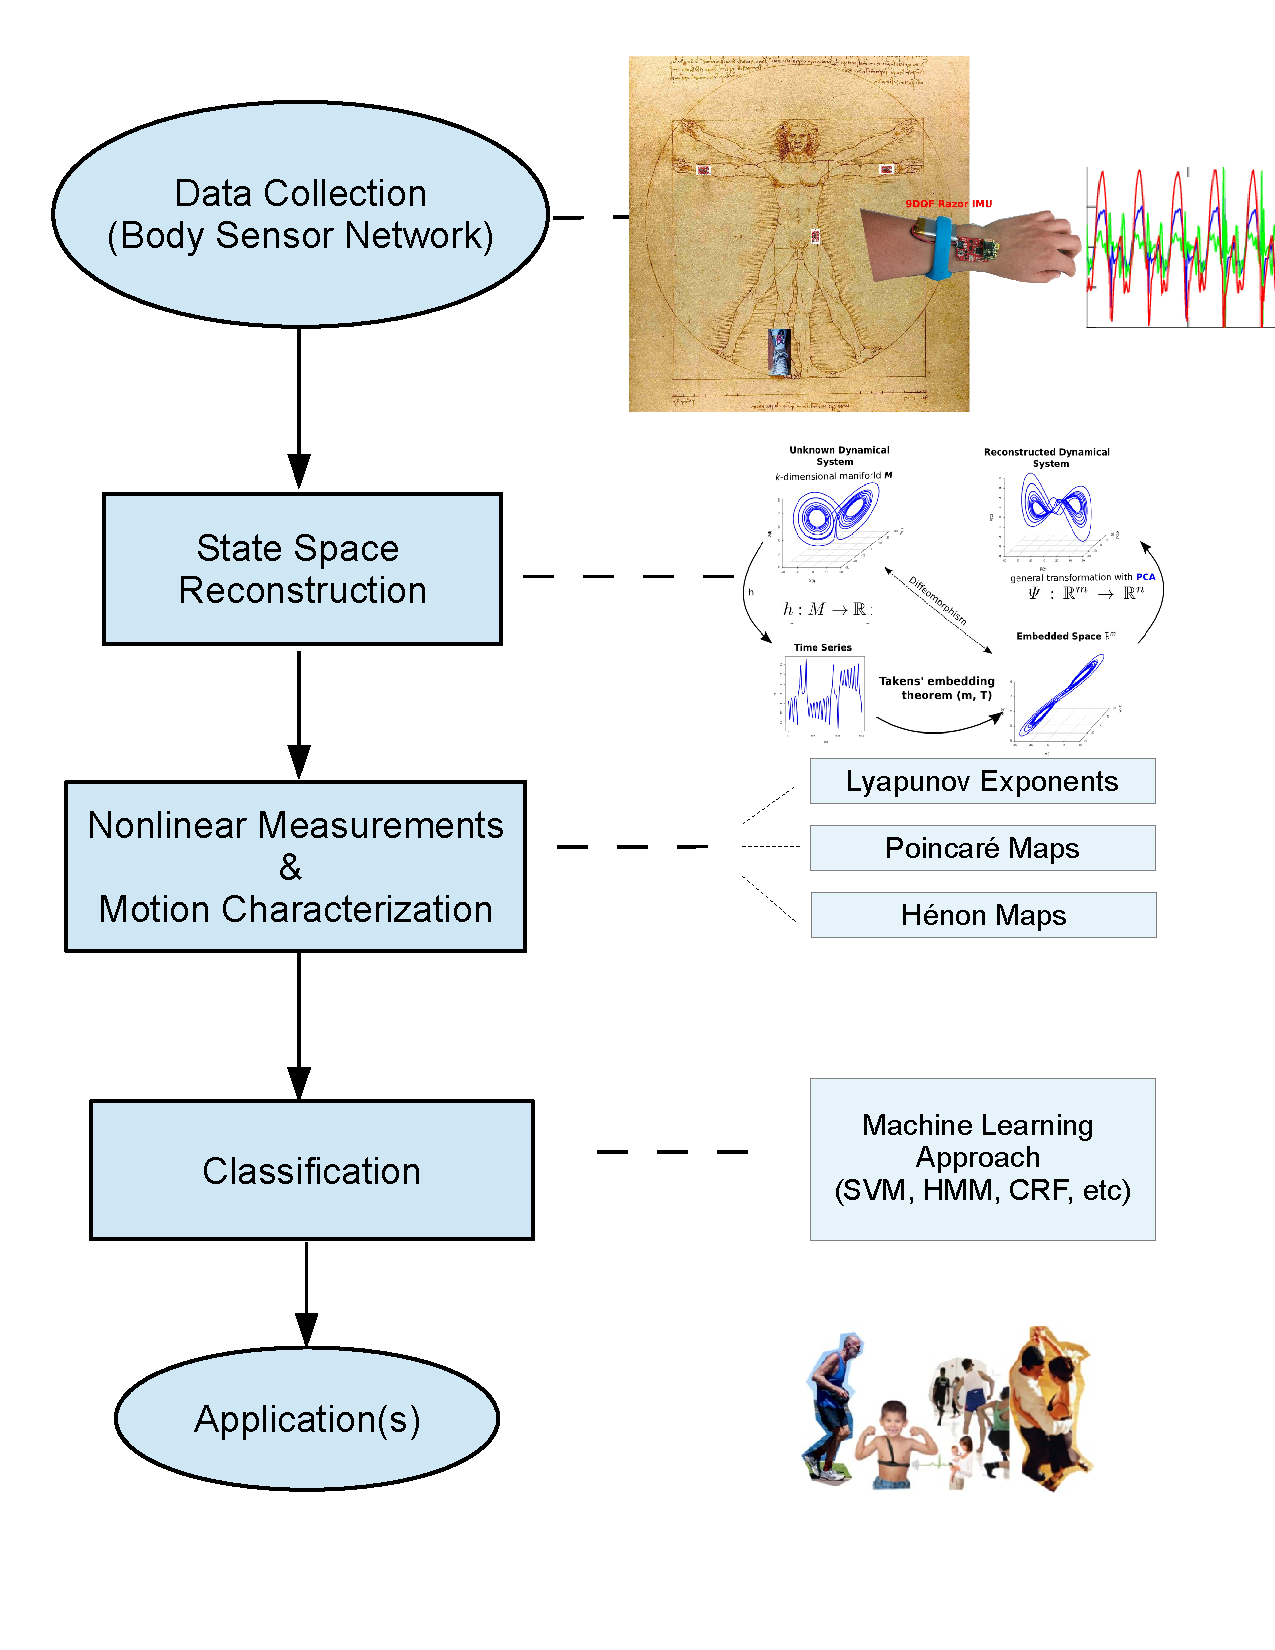
\includegraphics[width=0.9\textwidth]{proposedapproach_v1}
\caption[PA]{PhD Framework}
\label{fig:proposedapproach}
\end{figure}



Based on the proposed framework, 
tasks for the following 6 months are planned as follows:
\begin{itemize}[noitemsep,topsep=0pt,parsep=0pt,partopsep=0pt]
%  \item T1: 5 curses will be taken and they will be suggested by the doctoral committee.
\item T1 [February]: Review of state-of-the-art machine learning methods 
for human activity recognition using wearable sensors.
\item T2 [March]: Define the human activity experiment and recruit subjects 
to collect data so as to test the proposed PhD framework by means of a suitable
machine learning algorithm.
\item T4 [April]: Write and submit a paper in the 19th annual International Symposium
on Wearable Computers (Full/Note Paper Due: 10 April)
\item T5 [May-June]: Update the hardware of the body sensor network by using
Bluetooth low energy devices and inductive wireless chargers. 
\item T6 [May-June]: Update the open source sofware library for the body sensor
network.
\item T6 [July]: Write the 9th month report and create a publication
plan for the next year.
% \item T3: Definition of the experiments and motion capture system.
% \item T4: Programming method to obtain the reconstructed attractor
% \item T5: Evaluate the nonlinear measurements and the motion characterization.


% \item T9: Compare of the proposed approach with recent methods.
% \item T10 Writing, review and PhD thesis defence.
\end{itemize}

% Timeline is shown in the gantt chart 
% % (Figure \ref{fig:ganttchart})
% in which each year is divided into four periods (1 to 4).
% Additionally, it is an objective to write and publish at least two articles per year.
% 

% \begin{figure}[htbp!] 
% \begin{center}
%   \begin{gantt}{12}{12} %{rows}{columns}
%     \begin{ganttitle}
%       \numtitle{2014}{1}{2014}{1}
%       \numtitle{2015}{1}{2016}{4}
%       \numtitle{2017}{1}{2017}{3}
%     \end{ganttitle}
%     
%     \begin{ganttitle}
%       \numtitle{1}{1}{2}{1} % Titles with numbers
%       \numtitle{1}{1}{2}{1}
%       \numtitle{1}{1}{4}{1}
%       \numtitle{1}{1}{3}{1}
% %       \numtitle{1}{1}{3}{1}
%     \end{ganttitle}
%     
%   \ganttbar{T1}{0}{4}
%   \ganttbarcon{T2}{4}{2}
%   \ganttbarcon{T3}{5}{1}
%   \ganttbarcon{T4}{6}{2}
%   \ganttbarcon{T5}{6}{2}
%   \ganttbarcon{T6}{8}{1}
%   \ganttbarcon{T7}{8}{1}
%   \ganttbarcon{T8}{9}{1}
%   \ganttbarcon{T9}{9}{2}
%   \ganttbar{T10}{10}{2}
%   \end{gantt}
%   \caption[PA]{Gantt Chart for the research proposal}
% \label{fig:ganttchart}
%   \end{center}
% \end{figure}
  
  
  
 % Research Approach
% %*****************************************************************************************
%*********************************** Fourth Chapter **************************************
%*****************************************************************************************

\chapter{Timeline}

% **************************** Define Graphics Path **************************
\ifpdf
    \graphicspath{{Chapter4/Figs/Raster/}{Chapter4/Figs/PDF/}{Chapter4/Figs/}}
\else
    \graphicspath{{Chapter4/Figs/Vector/}{Chapter4/Figs/}}
\fi

Based on the proposed framework, tasks can be planned as follow:
\begin{itemize}[noitemsep,topsep=0pt,parsep=0pt,partopsep=0pt]
%  \item T1: 5 curses will be taken and they will be suggested by the doctoral committee.
 \item T2: State-of-the-art review in human activity recognition using 
 nonlinear dynamics.
% \item T3: Definition of the experiments and motion capture system.
% \item T4: Programming method to obtain the reconstructed attractor
% \item T5: Evaluate the nonlinear measurements and the motion characterization.
\item T6: Review of state-of-the-art of machine learning methods 
for human activity recognition using wearable sensors.
\item T7: Definition of the experiments and application(s).
\item T8: Selecting the subjects to test the application(s) in order to have 
data for publications.
\item T9: Comparison of the proposed approach with recent methods.
\item T10 Writing, review and PhD thesis defence.
\end{itemize}

Timeline is shown in the gantt chart (Figure \ref{fig:ganttchart})
in which each year is divided into four periods (1 to 4).
Additionally, it is an objective to write and publish at least two articles per year.


\begin{figure}[htbp!] 
\begin{center}
  \begin{gantt}{12}{12} %{rows}{columns}
    \begin{ganttitle}
      \numtitle{2014}{1}{2014}{1}
      \numtitle{2015}{1}{2016}{4}
      \numtitle{2017}{1}{2017}{3}
    \end{ganttitle}
    
    \begin{ganttitle}
      \numtitle{1}{1}{2}{1} % Titles with numbers
      \numtitle{1}{1}{2}{1}
      \numtitle{1}{1}{4}{1}
      \numtitle{1}{1}{3}{1}
%       \numtitle{1}{1}{3}{1}
    \end{ganttitle}
    
  \ganttbar{T1}{0}{4}
  \ganttbarcon{T2}{4}{2}
  \ganttbarcon{T3}{5}{1}
  \ganttbarcon{T4}{6}{2}
  \ganttbarcon{T5}{6}{2}
  \ganttbarcon{T6}{8}{1}
  \ganttbarcon{T7}{8}{1}
  \ganttbarcon{T8}{9}{1}
  \ganttbarcon{T9}{9}{2}
  \ganttbar{T10}{10}{2}
  \end{gantt}
  \caption[PA]{Gantt Chart for the research proposal}
\label{fig:ganttchart}
  \end{center}
\end{figure}
  
  
  
 % Timeline


% ********************************** Back Matter *******************************
% ********************************** Bibliography ******************************
%\backmatter 

\begin{spacing}{0.9}

% Bibliography style previews: http://nodonn.tipido.net/bibstyle.php
% \bibliographystyle{apalike}
\bibliographystyle{plainnat} % use this to have URLs listed in References

\cleardoublepage

\bibliography{References/references} % Path to your references.bib file

\end{spacing}

% ********************************** Appendices ********************************

\begin{appendices} % Using appendices environment for more functunality
% \include{Appendix1/appendix1}
\end{appendices}

% *************************************** Index ********************************
\printthesisindex %If index is present
\end{document}

